\documentclass[11pt]{article}

\usepackage{fancyhdr}
\usepackage{graphicx}
\usepackage{geometry}
\usepackage{lastpage}
\usepackage{titling}
\usepackage{sectsty}
\usepackage{setspace}
\usepackage{changepage}
\usepackage[shortlabels]{enumitem}
\usepackage{subcaption}
\usepackage{helvet}

\usepackage{tabularx}
\usepackage[table]{xcolor}
\usepackage{array}
\newcolumntype{P}[1]{>{\centering\arraybackslash}p{#1}}

\usepackage{siunitx}
\usepackage{nicefrac}
\usepackage{amsmath}
\usepackage{gensymb}
\usepackage{amssymb}
\usepackage{float}
\setcounter{MaxMatrixCols}{11}
\usepackage{indentfirst}

\usepackage{listings}
\usepackage{matlab-prettifier}
% \usepackage{color}
% \definecolor{dkgreen}{rgb}{0,0.6,0}
% \definecolor{gray}{rgb}{0.5,0.5,0.5}
% \definecolor{mauve}{rgb}{0.58,0,0.82}

\lstset
{
  frame=tb,
  style=Matlab-editor,
  % language=MATLAB, %Matlab-editor,
  aboveskip=3mm,
  belowskip=3mm,
  showstringspaces=false,
  columns=flexible,
  basicstyle={\small\ttfamily},
  numbers=none,
  % numberstyle=\tiny\color{gray},
  % keywordstyle=\color{blue},
  % commentstyle=\color{dkgreen},
  % stringstyle=\color{mauve},
  breaklines=true,
  breakatwhitespace=true,
  tabsize=3
}

\geometry
{
  letterpaper, 
  total={175.9mm,229.4mm}, 
  top=25mm, 
  left=20mm, 
  headheight=26pt,
  voffset=12pt,
  footskip=15pt
}
\author{Daniel Sturdivant}
\title{Lab 4}
\date{March 2023}
\graphicspath{ {./media/} }

\pagestyle{fancy}
\fancyhead[R]{March 17, 2023}
\fancyhead[L]{Sturdivant, Daniel \\ Weir, Andrew}
\fancyhead[C]{MECH 6970 GPS}
\fancyfoot[C]{Page \thepage\ of \pageref{LastPage}}

\makeatletter
\def\@maketitle
{
  \null
  \begin{center}
    {\huge \@title \\}
  \end{center}
  \vskip 5mm
}
\makeatother

\sectionfont{\fontsize{16}{16}}
\subsectionfont{\fontsize{13}{13}\normalfont}
\renewcommand{\thesubsection}{\arabic{section}-\arabic{subsection}}
\renewcommand{\familydefault}{\sfdefault}
\newcommand{\solution}{\textbf{Solution: \\}}


%% ====================================================================== %%
\begin{document}

\maketitle
\thispagestyle{fancy}
\setstretch{1.25}
% \setlength{\parskip}{0em}
% \setlength{\abovedisplayskip}{-8pt}
% \setlength{\belowdisplayskip}{12pt}
\setlength{\parindent}{0pt}

\begin{enumerate}[label=\textbf{\arabic*.}]
  \itemsep 24pt
    \item \textbf{Simple IF Data Analysis} \\
For this lab, IF data was used to generate a GPS position solution. The IF data used came from a IFEN SX3 with a 20000000 hertz sampling frequency and an intermediate frequency of 5000445.89 hertz. To analyze this data, 1 second of the IF data was pulled from the data file. The raw data values for the IF data between the times of 0.1 to 1 second are plotted in \emph{Figure 1}. 
    \begin{figure}[H]
        \centering
        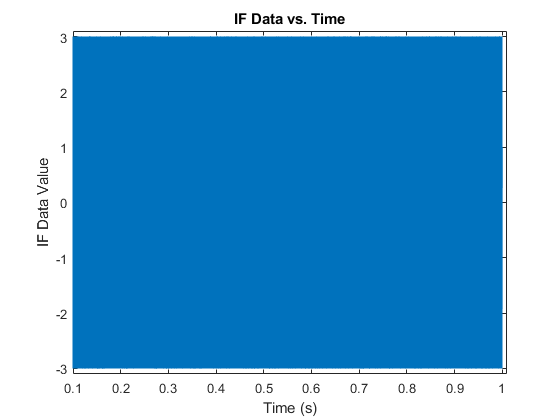
\includegraphics[width=0.85\textwidth]{Lab_4_IFEN_Time.png}
        \caption{IF Data Over Time.}
    \end{figure}
From \emph{Figure 1}, it can be seen that the IF data values vary between -3 and 3 across the entire time interval. Because the IF data is sampled at 20000000 hertz, however, it is hard to see any trends in the data at such a large time period. Therefore, \emph{Figure 2} shows a zoomed in plot of the IF data at a smaller 0.1 millimeter time period.
    \begin{figure}[H]
        \centering
        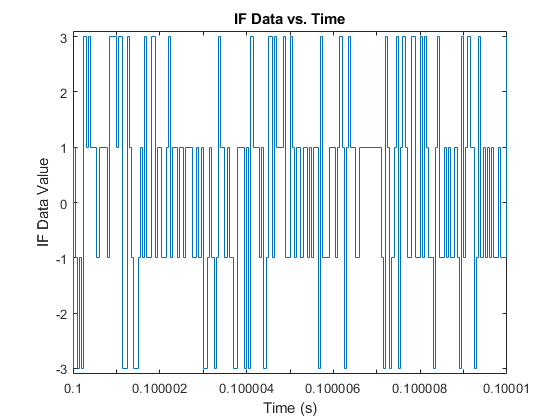
\includegraphics[width=0.85\textwidth]{Lab_4_IFEN_Time_2.png}
        \caption{IF Data Over Time Zoomed In.}
    \end{figure}
 Looking at the IF data at a smaller time interval shows a more legible depiction of the IF data. For most of the time period the IF data will vary between the values of -1 and 1. However, occasionally the IF data values will spike to either -3 or 3. Every single value of the IF data is either -3,-1,1 or 3 for the entire 1 second time period. This is better shown in the histogram of the IF data shown in \emph{Figure 3}. 
    \begin{figure}[H]
        \centering
        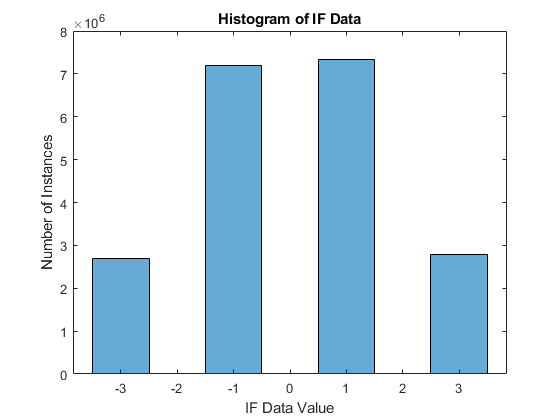
\includegraphics[width=0.85\textwidth]{Lab_4_IFEN_Hist.png}
        \caption{IF Data Histogram.}
    \end{figure}
From the histogram it can be seen that the most common values in the 1 second IF data set are -1 and 1. There are slightly more positive values than negative. This relationship is also true for the 3 values. Generally, for most instances of there being a positive value in the IF data a negative value also exists. However, there is no discernable pattern to these positive and negative values. Additionally, a power spectral analysis was performed on the IF data. \emph{Figure 4} shows the power spectral density of the 1 second of IF data.
    \begin{figure}[H]
        \centering
        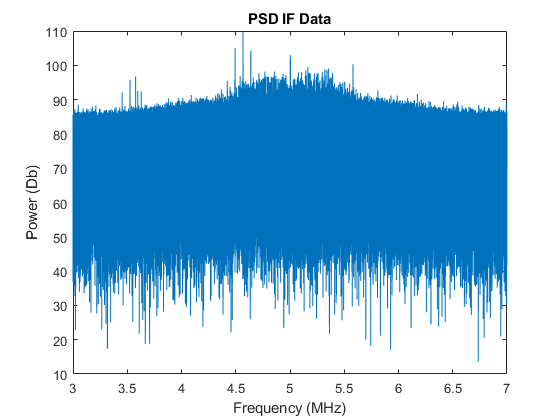
\includegraphics[width=0.85\textwidth]{Lab_4_IFEN_PSD.png}
        \caption{IF Data Power Spectral Density.}
    \end{figure}
The power spectral density shows a power spike around about 5 megahertz with the power at most other frequencies being the same. This spike in power corresponds to the intermediate frequency of the data. Another spike will occur at 15 megahertz after the data repeats. This is what we expect to happen for this set of IF data.

  \item \textbf{Satellite Acquisition} \\
The IF data is now used to acquire satellites. To do this, a Costas Phase lock loop (PLL) is used to determine the auto-correlation of the IF data at a range of different Doppler and code phases. The range of Doppler used was 10000 hertz above and below the intermediate frequency in 500 hertz intervals. The range of code phases used was the number of chips in a single PRN sequence. The correlation at each Doppler and code phase was calculated as a combination of the squares of the in-phase and quadrature. The equation to calculate the in-phase and quadrature for any given Doppler and code phase is given as:
    \begin{equation}
      I = S * CA * cos(2\pi\omega*t)
    \end{equation}
    \begin{equation}
      Q = S * CA * sin(2\pi\omega*t)
    \end{equation}
where $I$ is the the in-phase, $Q$ is the quadrature, $S$ is the IF signal, $CA$ is the shifted and up-sampled PRN sequence, $\omega$ is the Doppler frequency, and $t$ is the time vector. This methodology was used with 1 ms of data to try and acquire satellite 7. \emph{Figure 5} shows the resulting auto-correlation graph for satellite 7.
     \begin{figure}[H]
        \centering
        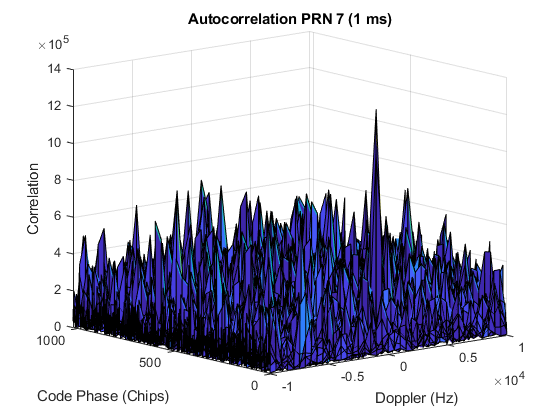
\includegraphics[width=0.85\textwidth]{Lab_4_PRN7_1ms.png}
        \caption{PRN 7 Acquisition 1 ms.}
    \end{figure}
It can be seen from this figure, that there is a noticeable spike in the correlation within this Doppler and code phase windows. Thus, satellite 7 was acquired within the 1 ms of data. The data would be much more uniform if satellite 7 was not available in this time period. This same process was repeated for 10 ms of data in \emph{Figure 6}.
    \begin{figure}[H]
        \centering
        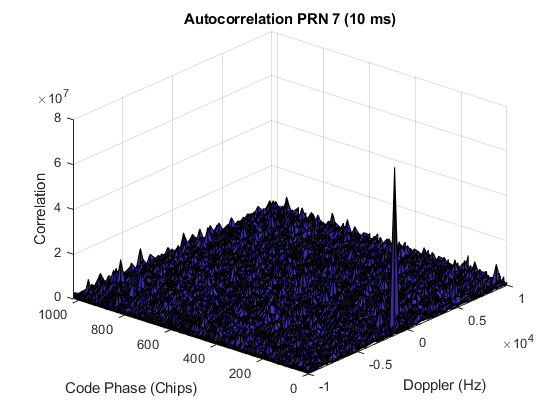
\includegraphics[width=0.85\textwidth]{Lab_4_PRN7_10ms.png}
        \caption{PRN 7 Acquisition 10 ms.}
    \end{figure}
Once again it is shown that satellite 7 has been acquired for this time interval. However, the correlation spike is much more prominent this time around. Increasing the amount of data in the correlation algorithm increases the performance of the acquisition. There is now much more confidence that satellite 7 has been acquired. \emph{Figure 7} shows auto-correlation for satellite 7 over the next 10 ms of data.
    \begin{figure}[H]
        \centering
        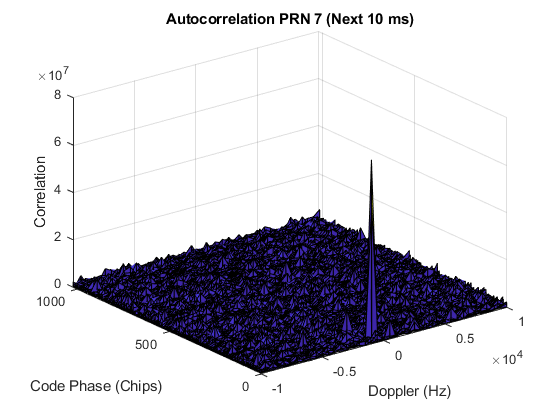
\includegraphics[width=0.85\textwidth]{Lab_4_PRN7_20ms.png}
        \caption{PRN 7 Acquisition Next 10 ms.}
    \end{figure}
Noise was then added to the data sequence with a standard deviation of 6. \emph{Figure 8} shows the resulting auto-correlation graph of the noisy measurement for satellite 7 over 1 ms of data.
    \begin{figure}[H]
        \centering
        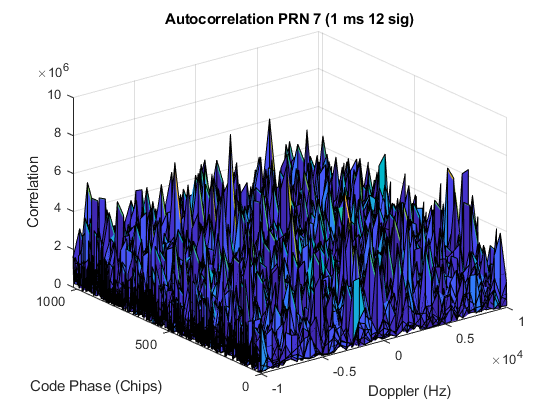
\includegraphics[width=0.85\textwidth]{Lab_4_PRN7_6sig_1ms.png}
        \caption{Noisy Satellite 7 (sigma=6) 1 ms.}
    \end{figure}
From the figure, it can be seen that the noise added to data sequence clouds the correlation solution. The peak in correlation is hidden amongst the correlation spikes due to the added noise. There is no longer an ability to acquire satellite 7 for this small time step. To improve the solution, a larger data size will need to be used. \emph{Figure 9} shows the auto-correlation graph for the same noise parameters but with 10 ms of data.
    \begin{figure}[H]
        \centering
        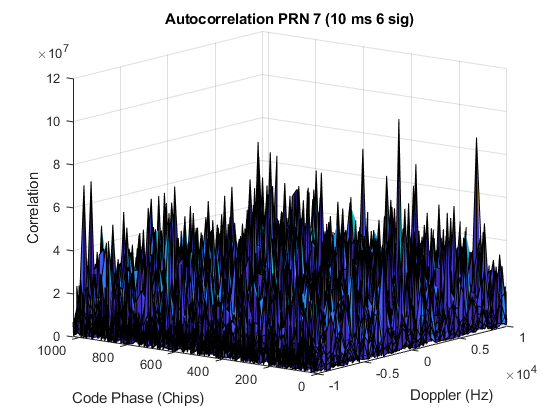
\includegraphics[width=0.85\textwidth]{Lab_4_PRN7_6sig_10ms.png}
        \caption{Noisy Satellite 7 (sigma=6) 10 ms.}
    \end{figure}
With the larger data size, the peak in correlation is much more pronounced. It is now possible to determine that satellite 7 has been acquired. The correlation spike is now larger than the noise floor with the larger data size. However, the performance of the acquisition code was much worse with the noisy signal. This same process was repeated but for a standard deviation value of 12. \emph{Figure 10} shows the auto-correlation of satellite 7 with the higher noise value for 1 ms of data.
    \begin{figure}[H]
        \centering
        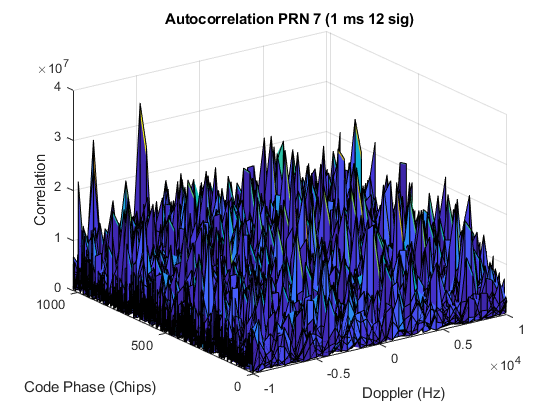
\includegraphics[width=0.85\textwidth]{Lab_4_PRN7_12sig_1ms.png}
        \caption{Noisy Satellite 7 (sigma=12) 1 ms.}
    \end{figure}
Once again, it is hard to identify a correlation spike amongst the noise for this small time period. Since the noise standard deviation value is higher, the correlation value is even more unidentifiable amongst the noise. Thus more data needs to be added for the satellite to be acquired. \emph{Figure 11} and \emph{Figure 12} show the auto-correlation graphs for 10 and 20 ms of noisy data respectively. 
    \begin{figure}[H]
        \centering
        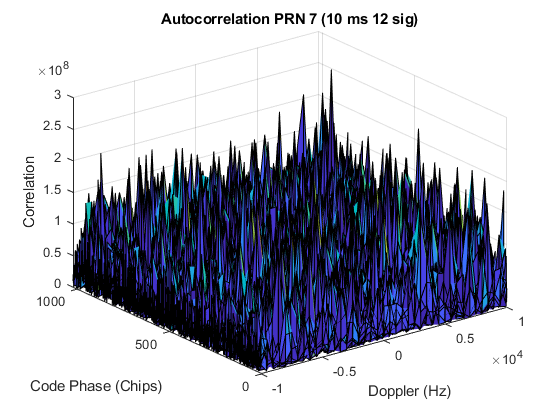
\includegraphics[width=0.85\textwidth]{Lab_4_PRN7_12sig_10ms.png}
        \caption{Noisy Satellite 7 (sigma=12) 10 ms.}
    \end{figure}
    \begin{figure}[H]
        \centering
        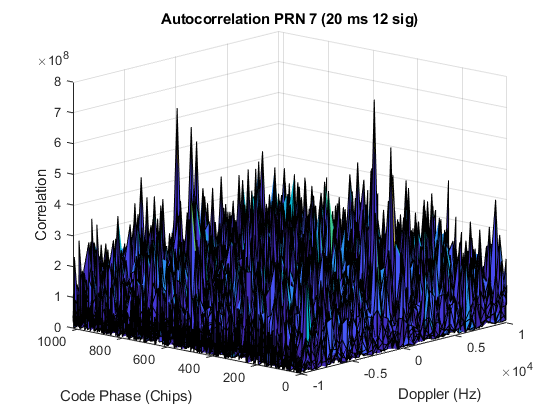
\includegraphics[width=0.85\textwidth]{Lab_4_PRN7_12sig_20ms.png}
        \caption{Noisy Satellite 7 (sigma=12) 20 ms.}
    \end{figure}
The increased noise makes it even harder to acquire satellite 7 with even 10 ms of data. It is still possible to see the correlation peak, but the noise clouds the result. When the amount of data is increased to 20 ms, however, the correlation peak is more visible. An increase in noise on the data, requires a subsequent increase in data size to acquire the satellite. This same satellite acquisition methodology was used to acquire more satellites over the 10 ms time period. \emph{Figures 13-17} show the auto-correlation graphs for satellites 1, 14, 17, 21, and 30 respectively.
    \begin{figure}[H]
        \centering
        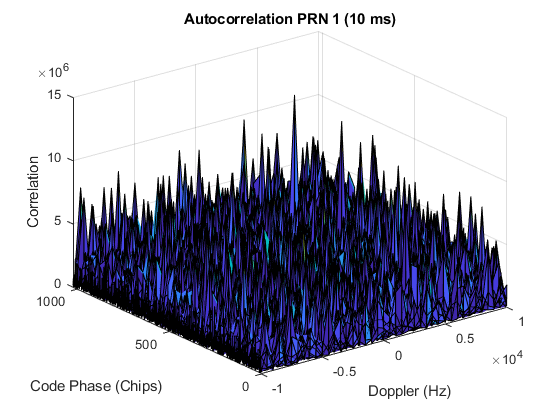
\includegraphics[width=0.75\textwidth]{Lab_4_PRN1_10ms.png}
        \caption{Satellite 1 Acquisition 10 ms.}
    \end{figure}
    \begin{figure}[H]
        \centering
        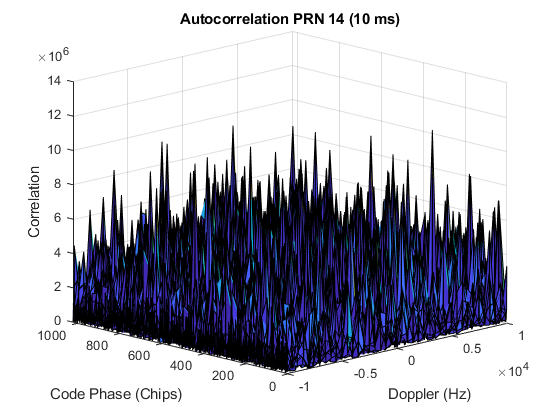
\includegraphics[width=0.75\textwidth]{Lab_4_PRN14_10ms.png}
        \caption{Satellite 14 Acquisition 10 ms.}
    \end{figure}
    \begin{figure}[H]
        \centering
        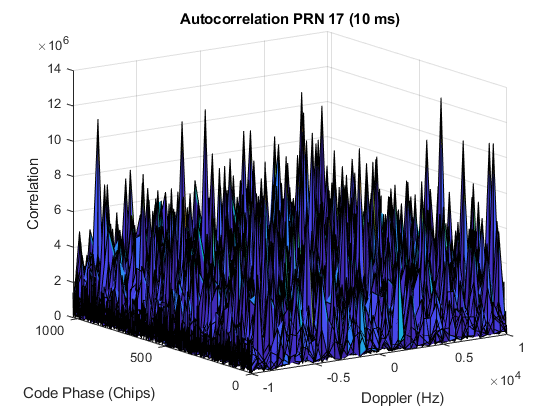
\includegraphics[width=0.75\textwidth]{Lab_4_PRN17_10ms.png}
        \caption{Satellite 17 Acquisition 10 ms.}
    \end{figure}
    \begin{figure}[H]
        \centering
        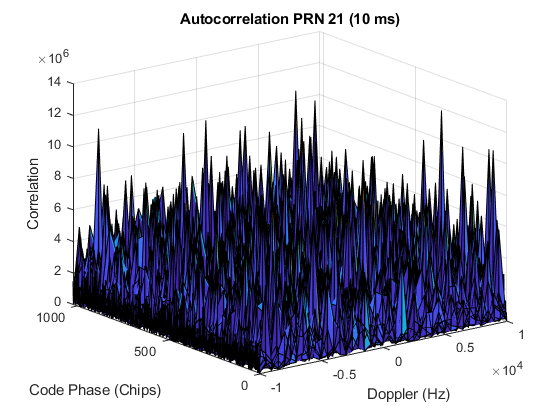
\includegraphics[width=0.75\textwidth]{Lab_4_PRN21_10ms.png}
        \caption{Satellite 21 Acquisition 10 ms.}
    \end{figure}
    \begin{figure}[H]
        \centering
        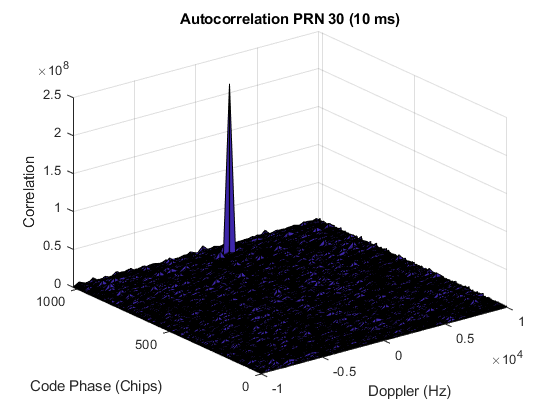
\includegraphics[width=0.75\textwidth]{Lab_4_PRN30_10ms.png}
        \caption{Satellite 30 Acquisition 10 ms.}
    \end{figure}
From the first 10 ms of data clear correlation spike can be seen for satellites 1 and 30. For these two satellites have been clearly acquired. Satellites 14 and 17 also have correlation peaks, but they are a lot less apparent than the other 3 satellites. No correlation spike is seen for satellite 21 for this time period. This same process was repeated for the next 10 ms of data. The results are seen in \emph{Figures 18-22}.
    \begin{figure}[H]
        \centering
        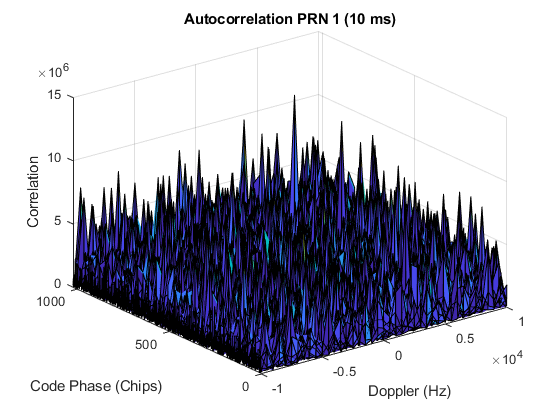
\includegraphics[width=0.75\textwidth]{Lab_4_PRN1_10ms.png}
        \caption{Satellite 1 Acquisition Next 10 ms.}
    \end{figure}
    \begin{figure}[H]
        \centering
        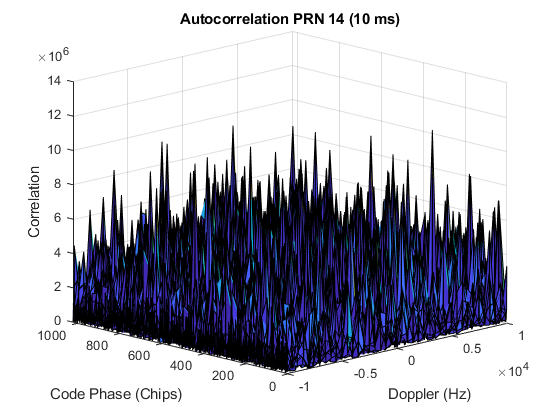
\includegraphics[width=0.75\textwidth]{Lab_4_PRN14_10ms.png}
        \caption{Satellite 14 Acquisition Next 10 ms.}
    \end{figure}
    \begin{figure}[H]
        \centering
        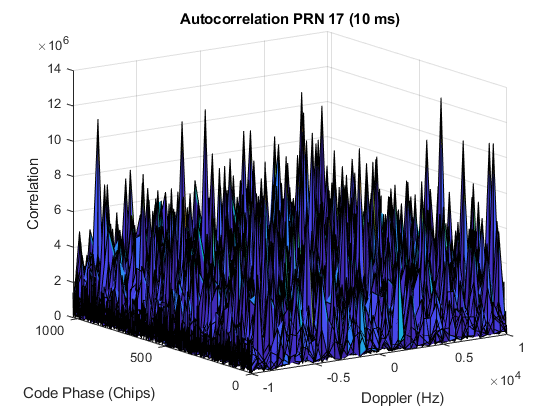
\includegraphics[width=0.75\textwidth]{Lab_4_PRN17_10ms.png}
        \caption{Satellite 17 Acquisition Next 10 ms.}
    \end{figure}
    \begin{figure}[H]
        \centering
        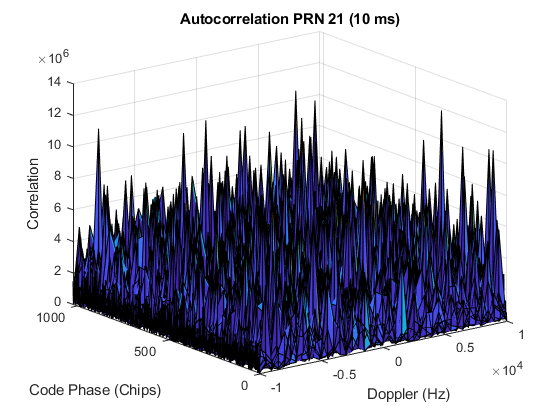
\includegraphics[width=0.75\textwidth]{Lab_4_PRN21_10ms.png}
        \caption{Satellite 21 Acquisition Next 10 ms.}
    \end{figure}
    \begin{figure}[H]
        \centering
        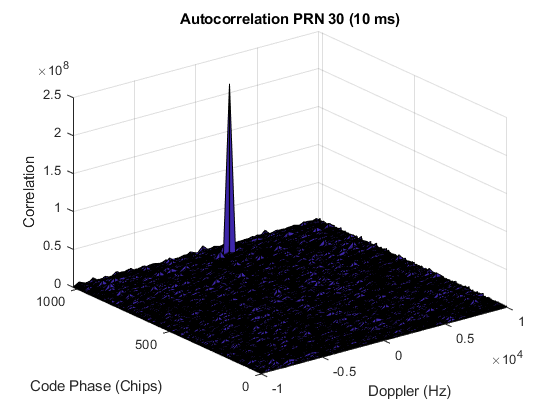
\includegraphics[width=0.75\textwidth]{Lab_4_PRN30_10ms.png}
        \caption{Satellite 30 Acquisition Next 10 ms.}
    \end{figure}
For this next 10 ms of data correlation peaks can now be seen for each of the satellites. The peaks for satellites 14 and 17 become more pronounced, and satellite 21 gains a peak. Satellites 1, 7, 14, 17, 21, and 30 have all been acquired for the first 20 ms of data. This is now more than enough satellites to get a position solution.
\end{enumerate}

    
\end{document}